\documentclass[CTN,authoryear,toc]{lsstdoc}
\input{meta}

% Package imports go here.
\usepackage{longtable}
\usepackage{url}
% Local commands go here.

%If you want glossaries
%\input{aglossary.tex}
%\makeglossaries

\title{LSSTCam and ComCam Focal Plane Layouts}

% This can write metadata into the PDF.
% Update keywords and author information as necessary.
\hypersetup{
    pdftitle={LSSTCam and ComCam Focal Plane Layouts},
    pdfauthor={First Last},
    pdfkeywords={}
}

% Optional subtitle
% \setDocSubtitle{A subtitle}

\input{authors}

\setDocRef{CTN-001}
\setDocUpstreamLocation{\url{https://github.com/lsst/ctn-001}}

\date{\vcsDate}

% Optional: name of the document's curator
% \setDocCurator{The Curator of this Document}

\setDocAbstract{%
This document includes figures depicting the layouts of the LSST Camera and ComCam, highlighting the arrangement and identification of science, wavefront, and guider sensors, as well as their individual readout image segments.
}

% Change history defined here.
% Order: oldest first.
% Fields: VERSION, DATE, DESCRIPTION, OWNER NAME.
% See LPM-51 for version number policy.
\setDocChangeRecord{%
  \addtohist{1}{2025-02-27}{Create document.}{Andrés A. Plazas Malagón, Seth Digel}
  \addtohist{1.1}{2025-03-15}{Add ComCam.}{Andrés A. Plazas Malagón, Seth Digel}
  \addtohist{1.2}{2025-05-20}{Add treering center}{HyeYun Park, Yousuke Utsumi}  
}

\begin{document}

% Create the title page.
\maketitle
% Frequently for a technote we do not want a title page  uncomment this to remove the title page and changelog.
% use \mkshorttitle to remove the extra pages

% ADD CONTENT HERE
% You can also use the \input command to include several content files.

\section{Focal Plane Layouts}
This document provides an overview of the LSSTCam and ComCam focal plane layouts.
Figures \ref{fig:focal_plane_1} and \ref{fig:focal_plane_2} below illustrate the placement of science, wavefront, and guider sensors of the LSST Camera, from both ITL and e2v.
The view is looking down from above the focal plane, i.e., through the LSSTCam lenses.

Figure \ref{fig:focal_plane_2} also includes the serial numbers of the raft tower modules (RTM-\#\#\#), the corner raft tower modules (CRTM-\#\#\#), and the individual CCDs.
The latter are the three-digit numbers immediately below the positional designator of the CCD.
For example, R11\_S10 is E2V-CCD-354) and R20\_S10 is ITL-CCD-351.
The raft and CCD serial numbers come from the \emph{eTraveler} database accessed using {\tt{datacat-utilities}}\footnote{\url{https://github.com/lsst-camera-dh/datacat-utilities}}.
Appendix A tabulates the mapping of raft and sensor slots to serial numbers.

The set of dead segments and high-noise segments is somewhat dynamic; dead or high-noise segments sometimes revive/recover and functioning segments sometimes die or become noisy.
The set of bad segments indicated in the figures is current as of the end of Run 7 electro-optical testing.
The corners of the treering centers are also displayed; for clarity, the markers are shown slightly inside each sensor, though the actual centers lie just outside the sensors.

Figure \ref{fig:focal_plane_3} shows the LSSTCam photographed in the LSST clean room, with the camera rotated 90 deg clockwise with respect to the diagrams in Figures \ref{fig:focal_plane_1} and \ref{fig:focal_plane_2}.
For more comprehensive technical details on the layout of the CCDs in the focal plane, consult the reference document \citeds{LCA-13381}

Corresponding diagrams and a photo for ComCam are shown in Figures \ref{fig:comcam_focal_plane_1}, \ref{fig:comcam_focal_plane_2}, and \ref{fig:comcam_focal_plane_3}. 

The source code used to generate the figures is available in the GitHub repository associated with this Camera Technical Note.

\clearpage

\begin{figure}
  \centering
  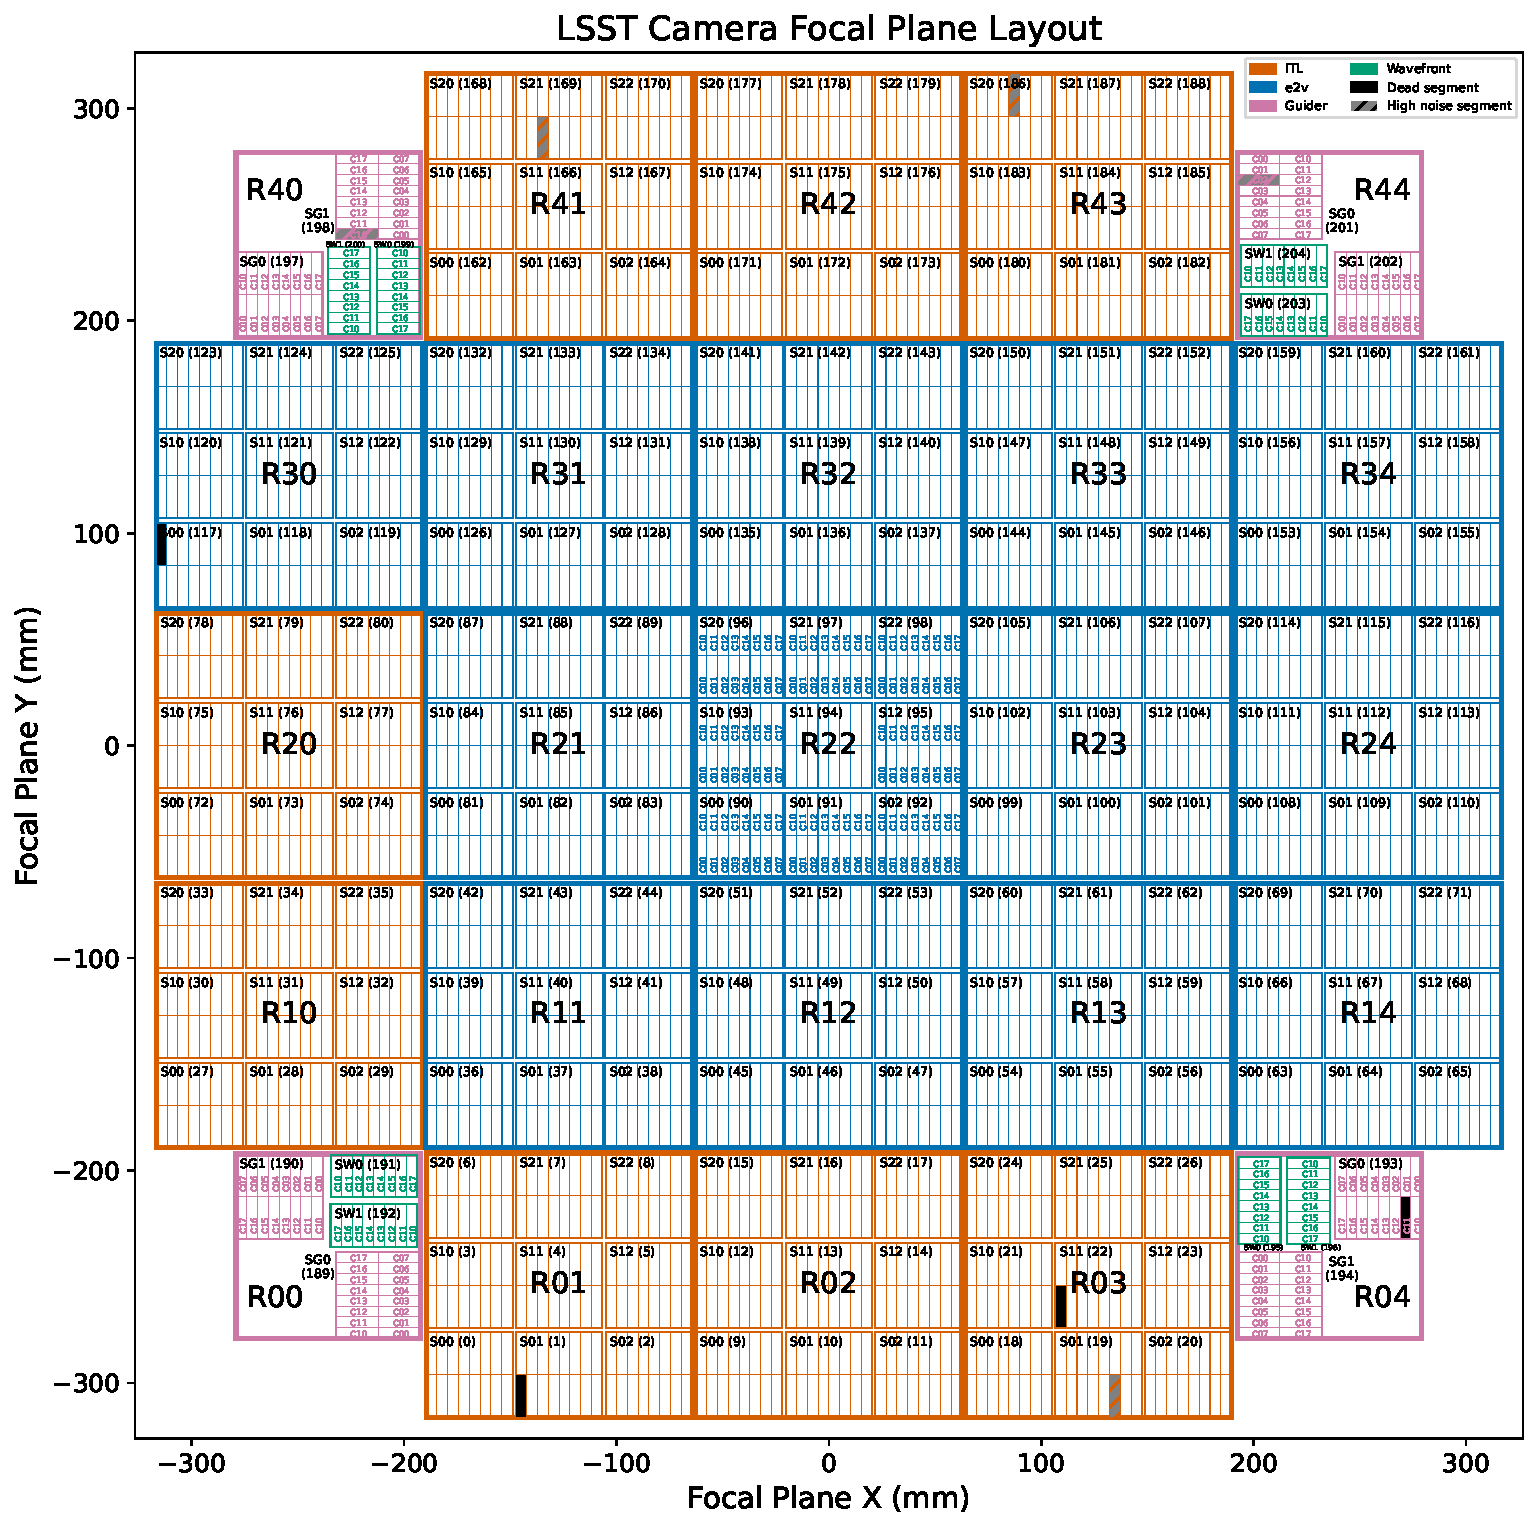
\includegraphics[width=\textwidth]{figures/LSSTCam_focal_plane_CTN_001_FIG1.pdf}
  \caption{LSSTCam focal plane layout. The following amplifiers (segments) are identified as either ``dead" or ``sometimes dead" due to readout noise being less than $4\,\mathrm{e}^{-}$ or an anomalous Photon Transfer Curve gain: {\tt{R30\_S00\_C10}}, {\tt{R01\_S01\_C00}}, {\tt{R03\_S11\_C00}}, {\tt{R04\_SG0\_C11}}. Additionally, the following amplifiers exhibit high readout noise ($> 18\,\mathrm{e}^{-}$): {\tt{R41\_S21\_C02}}, {\tt{R43\_S20\_C14}}, {\tt{R03\_S01\_C05}}, {\tt{R40\_SG1\_C10}}, {\tt{R44\_SG0\_C02}}. These classifications are based on Tables~8 and 9 of \citeds{SITCOMTN-148}. Code source: \url{https://github.com/lsst/ctn-001}}
  \label{fig:focal_plane_1}
\end{figure}

\clearpage

\begin{figure}
  \centering
  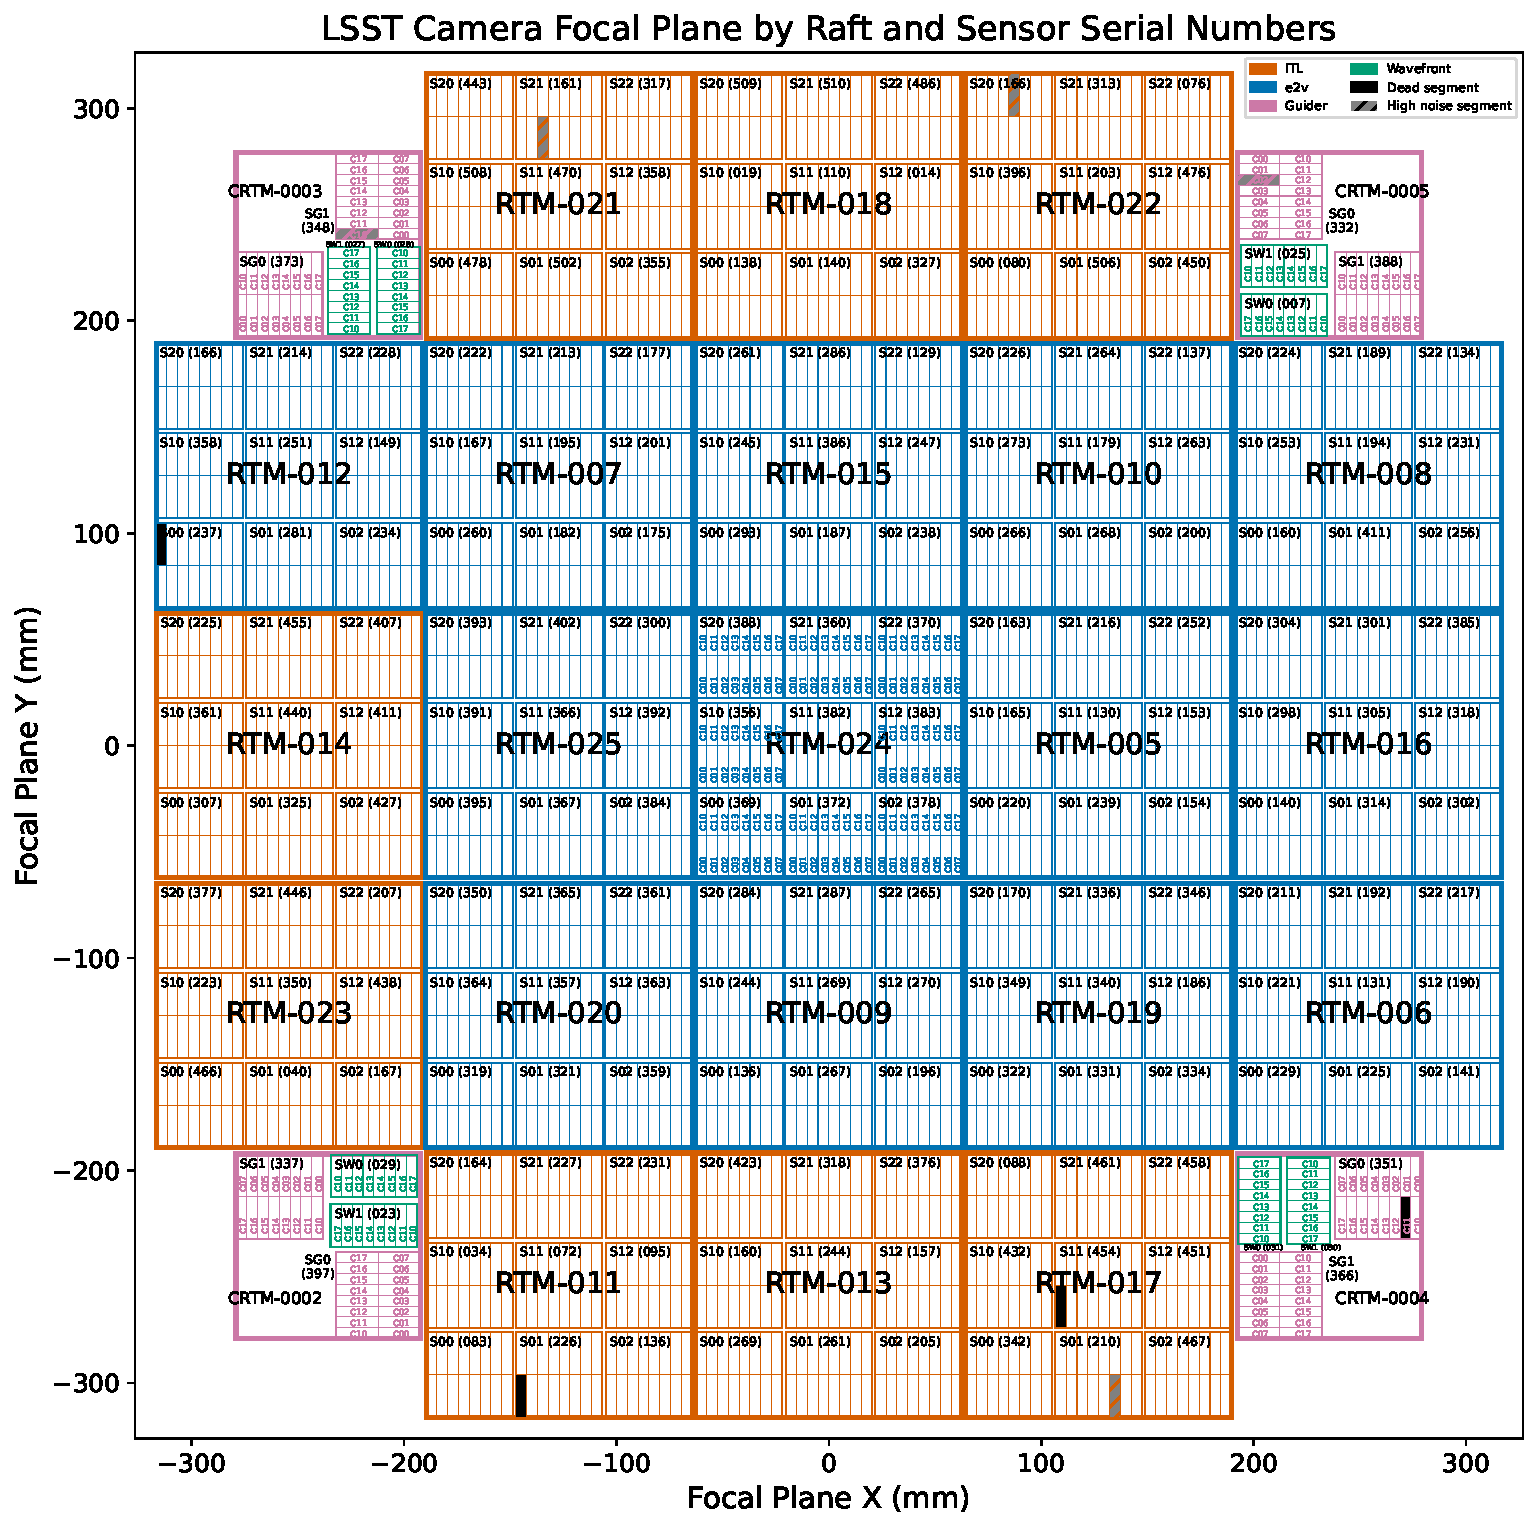
\includegraphics[width=\textwidth]{figures/LSSTCam_focal_plane_CTN_001_FIG2.pdf}
	\caption{LSSTCam focal plane layout including raft and CCD serial numbers (see text). The raft and CCD serial numbers come from the \emph{eTraveler} database accessed using {\tt{datacat-utilities}} (\url{https://github.com/lsst-camera-dh/datacat-utilities}). The bad segment list is as in~\ref{fig:focal_plane_1}.}
  \label{fig:focal_plane_2}
\end{figure}

\clearpage

\begin{figure}
  \centering
  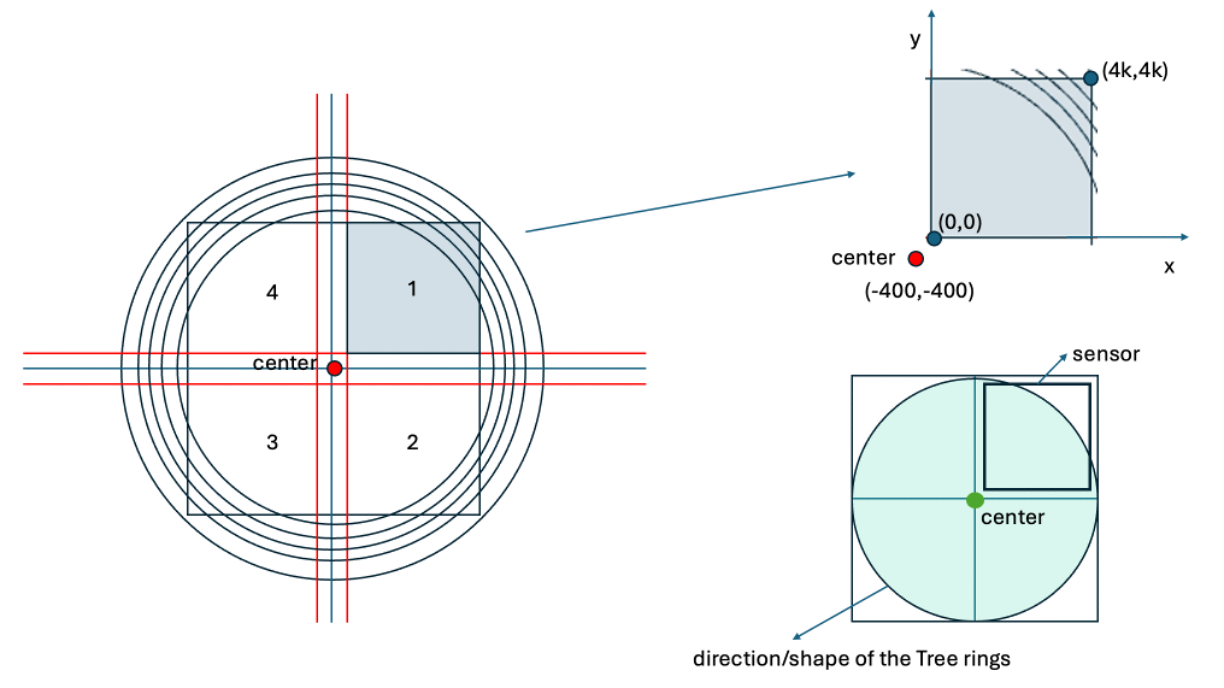
\includegraphics[width=\textwidth]{figures/TR_center_direction.png}
	\caption{The green dot in Figure \ref{fig:focal_plane_2} shows the center of Tree rings pattern, and it depends on which part of the wafer it is used to make the sensor. Direction of the Tree rings according to which corner the center is, is shown in this figure.}
  \label{fig:TR_direction_center}
\end{figure}

\begin{figure}
  \centering
  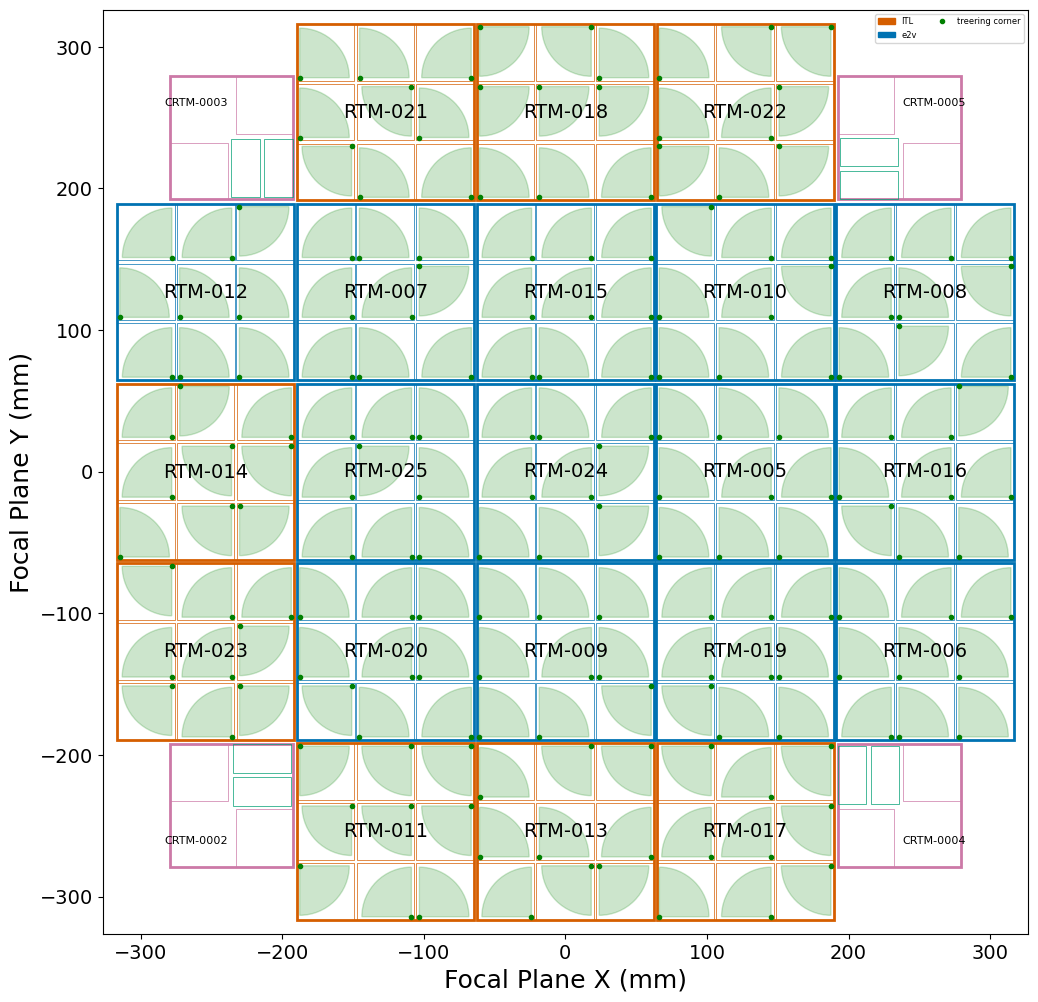
\includegraphics[width=\textwidth]{figures/Tree_ring_direction_center.png}
	\caption{The center of the Tree ring and the pattern direction for all sensors in LSSTCam}
  \label{fig:Focal_Plane_TR}
\end{figure}

\clearpage
\begin{figure}
  \centering
  \includegraphics[width=\textwidth]{figures/LSSTCam_photo.jpg}
  \caption{LSSTCam photographed in the LSST clean room on January 16, 2024. (Jacqueline Ramseyer Orrell/SLAC National Accelerator Laboratory). The camera is rotated 90 deg counter-clockwise with respect to the diagrams in Figures \ref{fig:focal_plane_1} and \ref{fig:focal_plane_2}. Image and caption source: \url{https://rubinobservatory.org/gallery/}}
  \label{fig:focal_plane_3}
\end{figure}


\begin{figure}
  \centering
  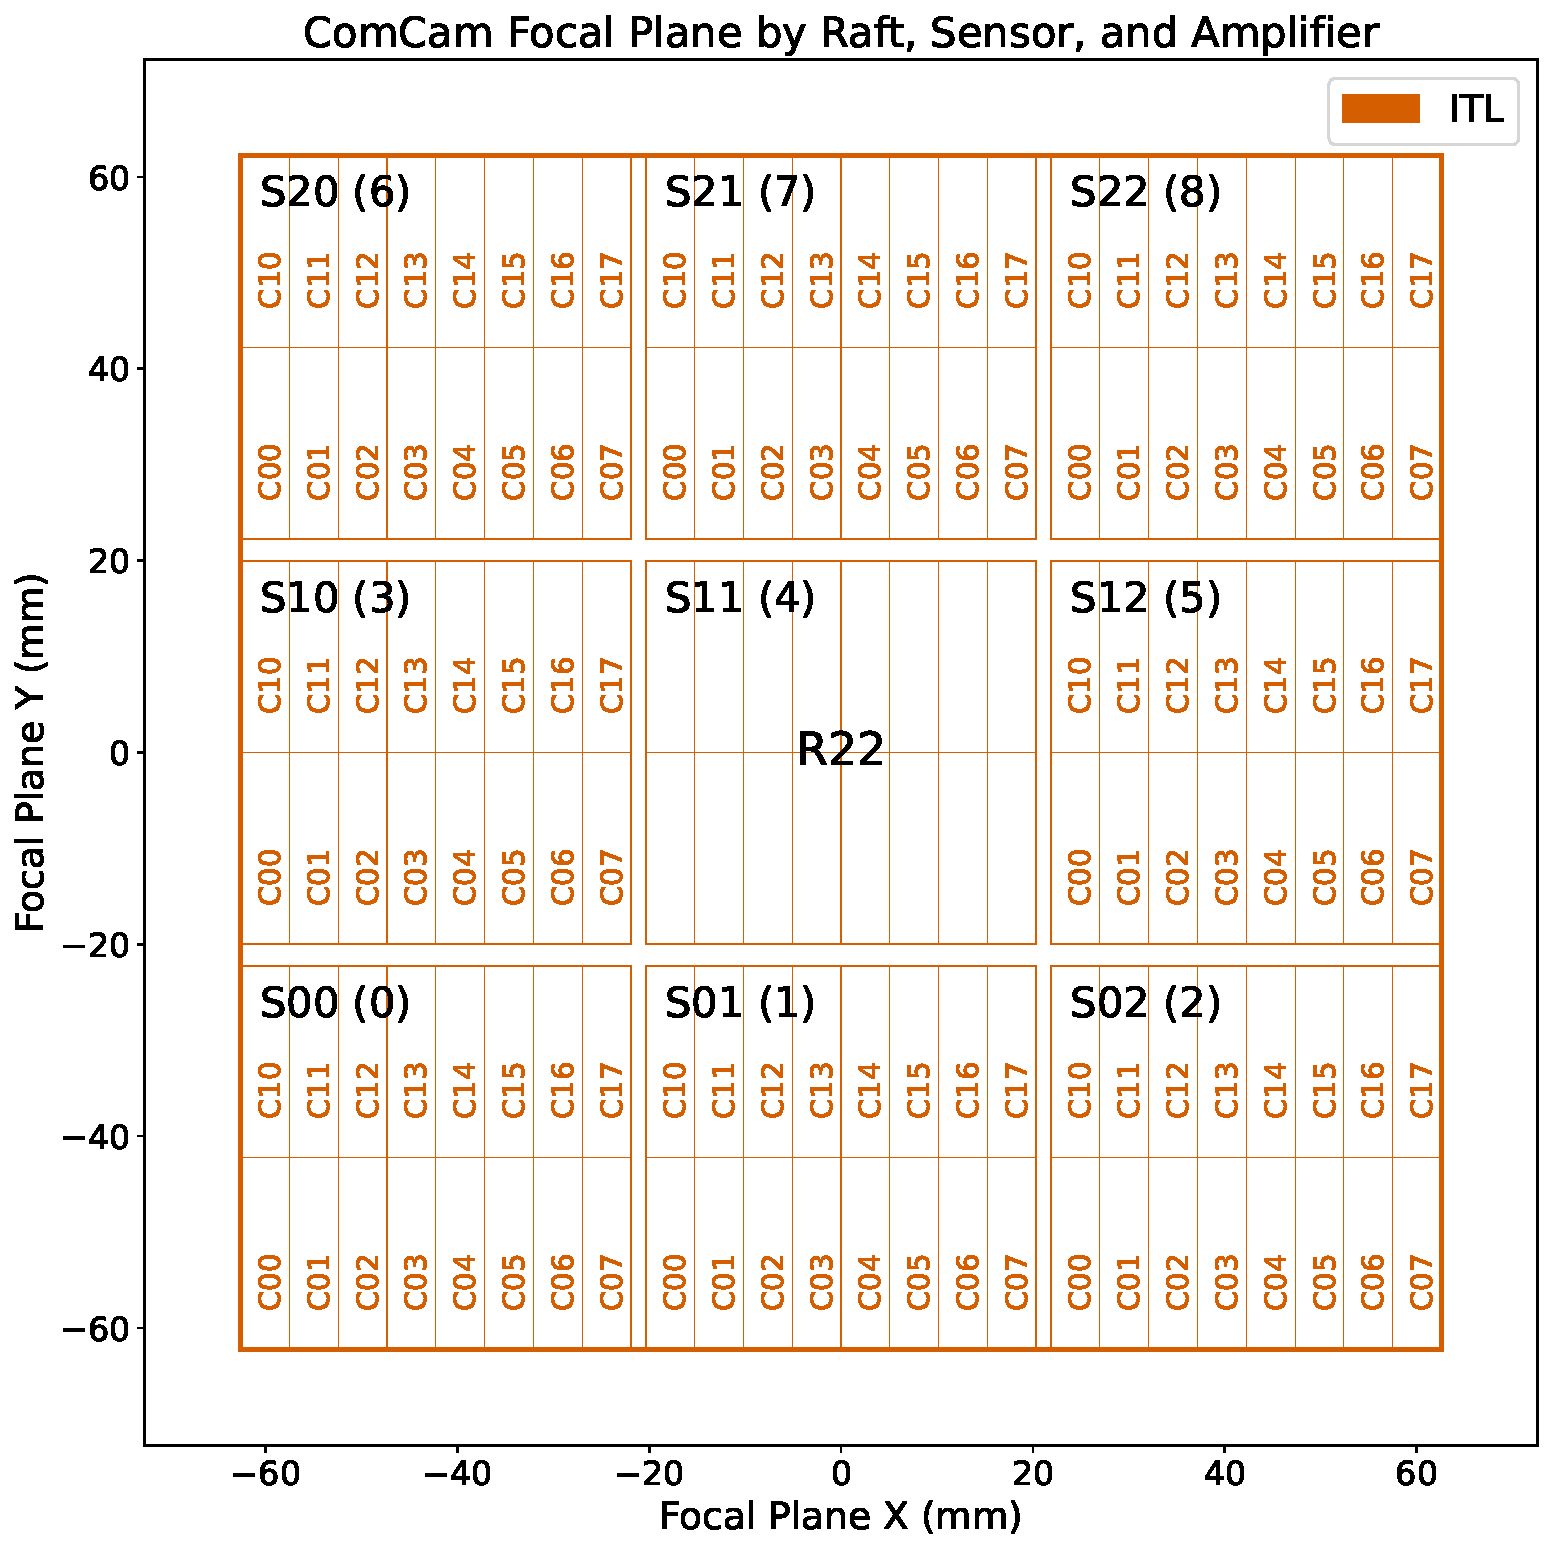
\includegraphics[width=\textwidth]{figures/ComCam_focal_plane_CTN_001_FIG1.pdf}
  \caption{ComCam focal plane layout. Code source: \url{https://github.com/lsst/ctn-001}}
  \label{fig:comcam_focal_plane_1}
\end{figure}

\clearpage

\begin{figure}
  \centering
  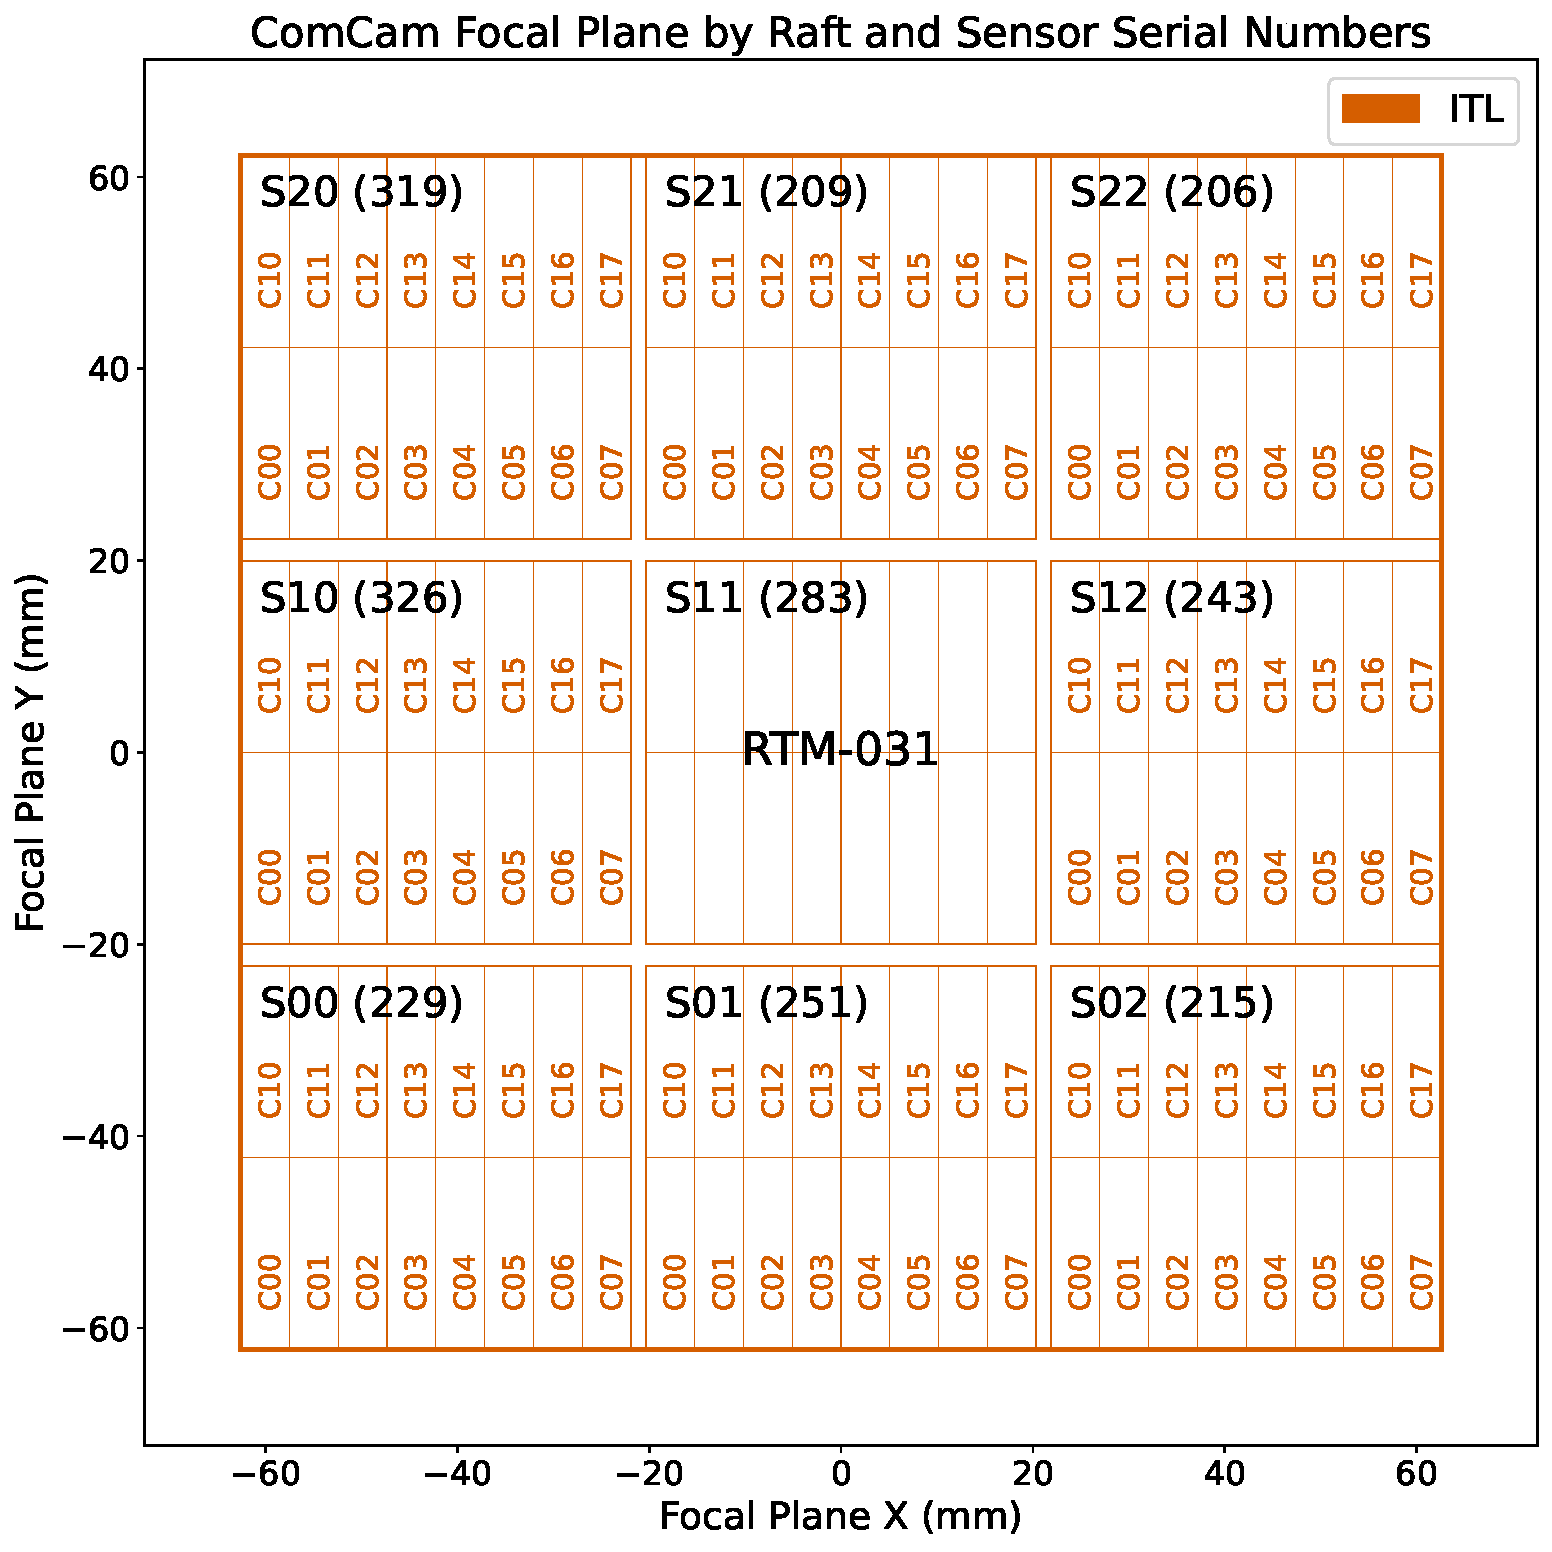
\includegraphics[width=\textwidth]{figures/ComCam_focal_plane_CTN_001_FIG2.pdf}
	\caption{ComCam focal plane layout including raft and CCD serial numbers (see text). The raft and CCD serial numbers come from the \emph{eTraveler} database accessed using {\tt{datacat-utilities}} (\url{https://github.com/lsst-camera-dh/datacat-utilities}).}
  \label{fig:comcam_focal_plane_2}
\end{figure}

\clearpage

\begin{figure}
  \centering
  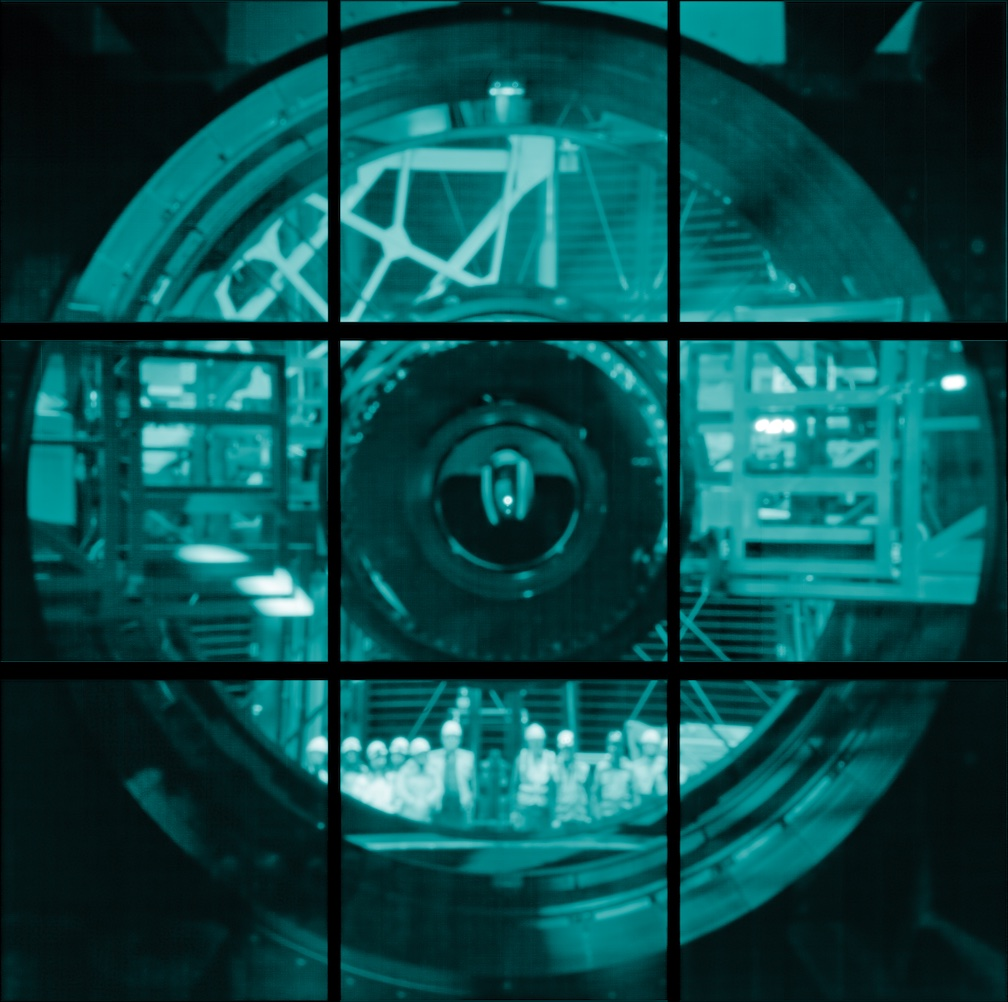
\includegraphics[width=\textwidth]{figures/comcam_photo.jpg}
  \caption{In one of the early images taken with Rubin's 144-megapixel test camera, Rubin staff gathered for a group photo inside the observatory dome, with the Simonyi Survey Telescope pointed at horizon. This "pinhole" image was created using the camera's sensors but without using lenses or mirrors to focus light. Instead of forming a detailed, zoomed-in picture, this technique gives a soft, unfocused image. The visible grid pattern of the camera's sensor array overlays the image. Image and caption source: \url{https://rubinobservatory.org/gallery/}}
  \label{fig:comcam_focal_plane_3}
\end{figure}


\appendix
\appendix
\section{Raft and Sensor Serial Numbers}
Table~\ref{tab:mapping} provides the mapping between the rafts, corner rafts, sensors, and their respective serial numbers.  See the caption of the table for details.  The information for the table was extracted from the eTraveler database using the datacat-utilities\footnote{\url{https://github.com/lsst-camera-dh/datacat-utilities}}.

\begin{longtable}{ccc}

\multicolumn{3}{c}{\bf R00  CRTM-0002  ITL} \\
\hline
  SG0 & 189 & ITL-CCD-397 \\
  SG1 & 190 & ITL-CCD-337 \\
  SW0 & 191 & ITL-CCD-029 \\
  SW1 & 192 & ITL-CCD-023 \\
 & & \\
\multicolumn{3}{c}{\bf R01  RTM-011  ITL} \\
\hline
  S00 & 000 & ITL-CCD-083 \\
  S01 & 001 & ITL-CCD-226 \\
  S02 & 002 & ITL-CCD-136 \\
  S10 & 003 & ITL-CCD-034 \\
  S11 & 004 & ITL-CCD-072 \\
  S12 & 005 & ITL-CCD-095 \\
  S20 & 006 & ITL-CCD-164 \\
  S21 & 007 & ITL-CCD-227 \\
  S22 & 008 & ITL-CCD-231 \\
 & & \\
\multicolumn{3}{c}{\bf R02  RTM-013  ITL} \\
\hline
  S00 & 009 & ITL-CCD-269 \\
  S01 & 010 & ITL-CCD-261 \\
  S02 & 011 & ITL-CCD-205 \\
  S10 & 012 & ITL-CCD-160 \\
  S11 & 013 & ITL-CCD-244 \\
  S12 & 014 & ITL-CCD-157 \\
  S20 & 015 & ITL-CCD-423 \\
  S21 & 016 & ITL-CCD-318 \\
  S22 & 017 & ITL-CCD-376 \\
 & & \\
\multicolumn{3}{c}{\bf R03  RTM-017  ITL} \\
\hline
  S00 & 018 & ITL-CCD-342 \\
  S01 & 019 & ITL-CCD-210 \\
  S02 & 020 & ITL-CCD-467 \\
  S10 & 021 & ITL-CCD-432 \\
  S11 & 022 & ITL-CCD-454 \\
  S12 & 023 & ITL-CCD-451 \\
  S20 & 024 & ITL-CCD-088 \\
  S21 & 025 & ITL-CCD-461 \\
  S22 & 026 & ITL-CCD-458 \\
 & & \\
\multicolumn{3}{c}{\bf R04  CRTM-0004  ITL} \\
\hline
  SG0 & 193 & ITL-CCD-351 \\
  SG1 & 194 & ITL-CCD-366 \\
  SW0 & 195 & ITL-CCD-031 \\
  SW1 & 196 & ITL-CCD-030 \\
 & & \\
\multicolumn{3}{c}{\bf R10  RTM-023  ITL} \\
\hline
  S00 & 027 & ITL-CCD-466 \\
  S01 & 028 & ITL-CCD-040 \\
  S02 & 029 & ITL-CCD-167 \\
  S10 & 030 & ITL-CCD-223 \\
  S11 & 031 & ITL-CCD-350 \\
  S12 & 032 & ITL-CCD-438 \\
  S20 & 033 & ITL-CCD-377 \\
  S21 & 034 & ITL-CCD-446 \\
  S22 & 035 & ITL-CCD-207 \\
 & & \\
\multicolumn{3}{c}{\bf R11  RTM-020  E2V} \\
\hline
  S00 & 036 & E2V-CCD-319 \\
  S01 & 037 & E2V-CCD-321 \\
  S02 & 038 & E2V-CCD-359 \\
  S10 & 039 & E2V-CCD-364 \\
  S11 & 040 & E2V-CCD-357 \\
  S12 & 041 & E2V-CCD-363 \\
  S20 & 042 & E2V-CCD-350 \\
  S21 & 043 & E2V-CCD-365 \\
  S22 & 044 & E2V-CCD-361 \\
 & & \\
\multicolumn{3}{c}{\bf R12  RTM-009  E2V} \\
\hline
  S00 & 045 & E2V-CCD-136 \\
  S01 & 046 & E2V-CCD-267 \\
  S02 & 047 & E2V-CCD-196 \\
  S10 & 048 & E2V-CCD-244 \\
  S11 & 049 & E2V-CCD-269 \\
  S12 & 050 & E2V-CCD-270 \\
  S20 & 051 & E2V-CCD-284 \\
  S21 & 052 & E2V-CCD-287 \\
  S22 & 053 & E2V-CCD-265 \\
 & & \\
\multicolumn{3}{c}{\bf R13  RTM-019  E2V} \\
\hline
  S00 & 054 & E2V-CCD-322 \\
  S01 & 055 & E2V-CCD-331 \\
  S02 & 056 & E2V-CCD-334 \\
  S10 & 057 & E2V-CCD-349 \\
  S11 & 058 & E2V-CCD-340 \\
  S12 & 059 & E2V-CCD-186 \\
  S20 & 060 & E2V-CCD-170 \\
  S21 & 061 & E2V-CCD-336 \\
  S22 & 062 & E2V-CCD-346 \\
 & & \\
\multicolumn{3}{c}{\bf R14  RTM-006  E2V} \\
\hline
  S00 & 063 & E2V-CCD-229 \\
  S01 & 064 & E2V-CCD-225 \\
  S02 & 065 & E2V-CCD-141 \\
  S10 & 066 & E2V-CCD-221 \\
  S11 & 067 & E2V-CCD-131 \\
  S12 & 068 & E2V-CCD-190 \\
  S20 & 069 & E2V-CCD-211 \\
  S21 & 070 & E2V-CCD-192 \\
  S22 & 071 & E2V-CCD-217 \\
 & & \\
\multicolumn{3}{c}{\bf R20  RTM-014  ITL} \\
\hline
  S00 & 072 & ITL-CCD-307 \\
  S01 & 073 & ITL-CCD-325 \\
  S02 & 074 & ITL-CCD-427 \\
  S10 & 075 & ITL-CCD-361 \\
  S11 & 076 & ITL-CCD-440 \\
  S12 & 077 & ITL-CCD-411 \\
  S20 & 078 & ITL-CCD-225 \\
  S21 & 079 & ITL-CCD-455 \\
  S22 & 080 & ITL-CCD-407 \\
 & & \\
\multicolumn{3}{c}{\bf R21  RTM-025  E2V} \\
\hline
  S00 & 081 & E2V-CCD-395 \\
  S01 & 082 & E2V-CCD-367 \\
  S02 & 083 & E2V-CCD-384 \\
  S10 & 084 & E2V-CCD-391 \\
  S11 & 085 & E2V-CCD-366 \\
  S12 & 086 & E2V-CCD-392 \\
  S20 & 087 & E2V-CCD-393 \\
  S21 & 088 & E2V-CCD-402 \\
  S22 & 089 & E2V-CCD-300 \\
 & & \\
\multicolumn{3}{c}{\bf R22  RTM-024  E2V} \\
\hline
  S00 & 090 & E2V-CCD-369 \\
  S01 & 091 & E2V-CCD-372 \\
  S02 & 092 & E2V-CCD-378 \\
  S10 & 093 & E2V-CCD-356 \\
  S11 & 094 & E2V-CCD-382 \\
  S12 & 095 & E2V-CCD-383 \\
  S20 & 096 & E2V-CCD-388 \\
  S21 & 097 & E2V-CCD-360 \\
  S22 & 098 & E2V-CCD-370 \\
 & & \\
\multicolumn{3}{c}{\bf R23  RTM-005  E2V} \\
\hline
  S00 & 099 & E2V-CCD-220 \\
  S01 & 100 & E2V-CCD-239 \\
  S02 & 101 & E2V-CCD-154 \\
  S10 & 102 & E2V-CCD-165 \\
  S11 & 103 & E2V-CCD-130 \\
  S12 & 104 & E2V-CCD-153 \\
  S20 & 105 & E2V-CCD-163 \\
  S21 & 106 & E2V-CCD-216 \\
  S22 & 107 & E2V-CCD-252 \\
 & & \\
\multicolumn{3}{c}{\bf R24  RTM-016  E2V} \\
\hline
  S00 & 108 & E2V-CCD-140 \\
  S01 & 109 & E2V-CCD-314 \\
  S02 & 110 & E2V-CCD-302 \\
  S10 & 111 & E2V-CCD-298 \\
  S11 & 112 & E2V-CCD-305 \\
  S12 & 113 & E2V-CCD-318 \\
  S20 & 114 & E2V-CCD-304 \\
  S21 & 115 & E2V-CCD-301 \\
  S22 & 116 & E2V-CCD-385 \\
 & & \\
\multicolumn{3}{c}{\bf R30  RTM-012  E2V} \\
\hline
  S00 & 117 & E2V-CCD-237 \\
  S01 & 118 & E2V-CCD-281 \\
  S02 & 119 & E2V-CCD-234 \\
  S10 & 120 & E2V-CCD-358 \\
  S11 & 121 & E2V-CCD-251 \\
  S12 & 122 & E2V-CCD-149 \\
  S20 & 123 & E2V-CCD-166 \\
  S21 & 124 & E2V-CCD-214 \\
  S22 & 125 & E2V-CCD-228 \\
 & & \\
\multicolumn{3}{c}{\bf R31  RTM-007  E2V} \\
\hline
  S00 & 126 & E2V-CCD-260 \\
  S01 & 127 & E2V-CCD-182 \\
  S02 & 128 & E2V-CCD-175 \\
  S10 & 129 & E2V-CCD-167 \\
  S11 & 130 & E2V-CCD-195 \\
  S12 & 131 & E2V-CCD-201 \\
  S20 & 132 & E2V-CCD-222 \\
  S21 & 133 & E2V-CCD-213 \\
  S22 & 134 & E2V-CCD-177 \\
 & & \\
\multicolumn{3}{c}{\bf R32  RTM-015  E2V} \\
\hline
  S00 & 135 & E2V-CCD-293 \\
  S01 & 136 & E2V-CCD-187 \\
  S02 & 137 & E2V-CCD-238 \\
  S10 & 138 & E2V-CCD-245 \\
  S11 & 139 & E2V-CCD-386 \\
  S12 & 140 & E2V-CCD-247 \\
  S20 & 141 & E2V-CCD-261 \\
  S21 & 142 & E2V-CCD-286 \\
  S22 & 143 & E2V-CCD-129 \\
 & & \\
\multicolumn{3}{c}{\bf R33  RTM-010  E2V} \\
\hline
  S00 & 144 & E2V-CCD-266 \\
  S01 & 145 & E2V-CCD-268 \\
  S02 & 146 & E2V-CCD-200 \\
  S10 & 147 & E2V-CCD-273 \\
  S11 & 148 & E2V-CCD-179 \\
  S12 & 149 & E2V-CCD-263 \\
  S20 & 150 & E2V-CCD-226 \\
  S21 & 151 & E2V-CCD-264 \\
  S22 & 152 & E2V-CCD-137 \\
 & & \\
\multicolumn{3}{c}{\bf R34  RTM-008  E2V} \\
\hline
  S00 & 153 & E2V-CCD-160 \\
  S01 & 154 & E2V-CCD-411 \\
  S02 & 155 & E2V-CCD-256 \\
  S10 & 156 & E2V-CCD-253 \\
  S11 & 157 & E2V-CCD-194 \\
  S12 & 158 & E2V-CCD-231 \\
  S20 & 159 & E2V-CCD-224 \\
  S21 & 160 & E2V-CCD-189 \\
  S22 & 161 & E2V-CCD-134 \\
 & & \\
\multicolumn{3}{c}{\bf R40  CRTM-0003  ITL} \\
\hline
  SG0 & 197 & ITL-CCD-373 \\
  SG1 & 198 & ITL-CCD-348 \\
  SW0 & 199 & ITL-CCD-028 \\
  SW1 & 200 & ITL-CCD-027 \\
 & & \\
\multicolumn{3}{c}{\bf R41  RTM-021  ITL} \\
\hline
  S00 & 162 & ITL-CCD-478 \\
  S01 & 163 & ITL-CCD-502 \\
  S02 & 164 & ITL-CCD-355 \\
  S10 & 165 & ITL-CCD-508 \\
  S11 & 166 & ITL-CCD-470 \\
  S12 & 167 & ITL-CCD-358 \\
  S20 & 168 & ITL-CCD-443 \\
  S21 & 169 & ITL-CCD-161 \\
  S22 & 170 & ITL-CCD-317 \\
 & & \\
\multicolumn{3}{c}{\bf R42  RTM-018  ITL} \\
\hline
  S00 & 171 & ITL-CCD-138 \\
  S01 & 172 & ITL-CCD-140 \\
  S02 & 173 & ITL-CCD-327 \\
  S10 & 174 & ITL-CCD-019 \\
  S11 & 175 & ITL-CCD-110 \\
  S12 & 176 & ITL-CCD-014 \\
  S20 & 177 & ITL-CCD-509 \\
  S21 & 178 & ITL-CCD-510 \\
  S22 & 179 & ITL-CCD-486 \\
 & & \\
\multicolumn{3}{c}{\bf R43  RTM-022  ITL} \\
\hline
  S00 & 180 & ITL-CCD-080 \\
  S01 & 181 & ITL-CCD-506 \\
  S02 & 182 & ITL-CCD-450 \\
  S10 & 183 & ITL-CCD-396 \\
  S11 & 184 & ITL-CCD-203 \\
  S12 & 185 & ITL-CCD-476 \\
  S20 & 186 & ITL-CCD-166 \\
  S21 & 187 & ITL-CCD-313 \\
  S22 & 188 & ITL-CCD-076 \\
 & & \\
\multicolumn{3}{c}{\bf R44  CRTM-0005  ITL} \\
\hline
  SG0 & 201 & ITL-CCD-332 \\
  SG1 & 202 & ITL-CCD-388 \\
  SW0 & 203 & ITL-CCD-007 \\
  SW1 & 204 & ITL-CCD-025 \\
 & & \\

    \caption{Each table lists the raft serial number (CRTM-\#\#\# or RTM-\#\#\#, and the CCD content of each raft.  For each CCD the slot S\#\# and DM index are listed along with the vendor's serial number.}
   \label{tab:mapping}
\end{longtable}
% Include all the relevant bib files.
% https://lsst-texmf.lsst.io/lsstdoc.html#bibliographies
\section{References} \label{sec:bib}
\renewcommand{\refname}{} % Suppress default Bibliography section
\bibliography{local,lsst,lsst-dm,refs_ads,refs,books}

% Make sure lsst-texmf/bin/generateAcronyms.py is in your path
\section{Acronyms} \label{sec:acronyms}
\addtocounter{table}{-1}
\begin{longtable}{p{0.145\textwidth}p{0.8\textwidth}}\hline
\textbf{Acronym} & \textbf{Description}  \\\hline

CCD & Charge-Coupled Device \\\hline
ITL & Imaging Technology Laboratory (UA) \\\hline
LCA & Document handle LSST camera subsystem controlled documents \\\hline
LSST & Legacy Survey of Space and Time (formerly Large Synoptic Survey Telescope) \\\hline
OPS & Operations \\\hline
RTM & Raft Tower Module \\\hline
SLAC & SLAC National Accelerator Laboratory \\\hline
\end{longtable}

% If you want glossary uncomment below -- comment out the two lines above
%\printglossaries





\end{document}
